\section{Introdución}
La seguridad ciudadana constituye uno de los principales problemas sociales de varios países de América Latina, cuyos ciudadanos están profundamente preocupados por el fuerte incremento en la tasa de criminalidad, se sienten cada vez más inseguros en sus personas y bienes, y expresan su insatisfacción con respecto a la respuesta estatal ante el fenómeno delictivo\cite{rico2002seguridad}.\\
El fenómeno delictivo es un tema complejo, y muchas veces parece que cualquier acción que se realice para prevenirlo o controlarlo resulta insuficiente. Para esto es fundamental desarrollar diagnósticos de calidad basados en indicadores válidos y confiables\cite{ensc2014}.\\
En Paraguay, la Policia Nacional cuenta con jefaturas zonales y departamentales. Las jefaturas departamentales se subdividen en comisarías. La ciudad de Asunción cuenta con veinticuatro (24) comisarias; éstas tienen a su cargo cuatro o cinco cuadrantes, en los que operan un vehículo con dos o tres policías y a su vez, cada cuadrante se subdivide en sectores\cite{ensc2014}. \\
En fecha del 18 de octubre de 2012, fue sancionada la Ley que crea el Sistema Nacional de Emergencias denominado 911, para la atención de comunicaciones de emergencias. El sistema 911 funciona en un moderno centro de comando y recibe aproximadamente 7 mil llamadas diarias. Para tal tarea, un total de 45 efectivos policiales trabajan en tres turnos en el centro de comando y dirigen la labor de 120 patrulleros en Asunción y 400 en el Gran Asunción -preliminarmente administrados por el 911 y ahora adscritos a las comisarías-, de los cuales solo 114 tienen GPS en la actualidad. Se calcula que cada vehículo recorre diariamente entre 100 y 150 kilómetros\cite{ensc2014}.\\
Las llamadas dirijidas al 911 pasan por 4 etapas de tiempos [\cref{fig:time1}], que están definidas como (1) recepción, (2) procesamiento, (3) asignación del recurso policial encargado y (4) desplazamiento del recurso asignado.
\begin{figure}[!h]
    \centering
    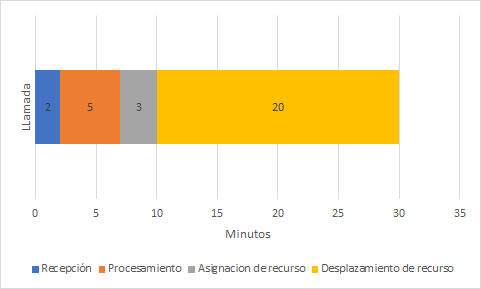
\includegraphics[width=100mm,scale=0.5]{images/tiempo_llamadas.png}
    \caption{Tiempo de vida promedio por llamada.}
    \label{fig:time1}
\end{figure}
\\A partir de lo citado anteriormente, se tomó como referencia el trabajo de [N. MENDES and A. SANTOS]\cite{mendesd} para obtener posiciones óptimas en la ubicación de los recursos policiales utilizando el procedimiento metaheurístico de la búsqueda Tabú. A fin de obtener valores más precisos fueron necesarios aplicar modificaciones al trabajo referenciado, los que serán detallados en las siguientes secciones.\\
Este trabajo, se enfoca en la optimización de la etapa 4 (desplazamiento del recurso) de las llamadas [\cref{fig:time1}], de tal forma a reducir al mínimo posible el tiempo transcurrido desde el inicio de la llamada hasta la asistencia del recurso policial, mediante la utilización del histórico de datos delictivos con georeferencias.